% !TEX program = xelatex
% Bien dich bang XeLaTeX (khong dung pdflatex), chay 2 lan de co so trang.
% Thu muc co san file latexmkrc: latexmk va LaTeX Workshop se tu goi xelatex.
\documentclass[aspectratio=169,11pt]{beamer}

\usepackage{fontspec}
\usepackage{xcolor}
\usepackage{listings}
\usepackage{booktabs}
\usepackage{array}
\usepackage{tikz}
\usetikzlibrary{positioning,arrows.meta,calc,fit,backgrounds}

% ===== Mau =====
\definecolor{chinh}{HTML}{1F3A5F}     % mau chu dao
\definecolor{nhan}{HTML}{C0392B}      % mau nhan manh trong code
\definecolor{nenma}{HTML}{F4F5F7}     % nen khung code
\definecolor{nenhop}{HTML}{EAF0F7}    % nen hop ket luan
\definecolor{xam}{HTML}{6B7280}
\definecolor{vien}{HTML}{C9CED6}
\definecolor{chuoi}{HTML}{2E7D32}

% ===== Giao dien beamer =====
\usetheme{default}
\setbeamertemplate{navigation symbols}{}
\setbeamersize{text margin left=9mm,text margin right=9mm}
\setbeamercolor{structure}{fg=chinh}
\setbeamercolor{frametitle}{fg=chinh}
\setbeamerfont{frametitle}{series=\bfseries,size=\Large}
\setbeamercolor{footline}{fg=xam}
\setbeamerfont{footline}{size=\scriptsize}
\setbeamertemplate{itemize item}{\raisebox{0.25ex}{\rule{0.75ex}{0.75ex}}}
\setbeamertemplate{itemize subitem}{\raisebox{0.35ex}{\rule{0.55ex}{0.55ex}}}
\setbeamertemplate{enumerate item}{\insertenumlabel.}
\setlength{\leftmargini}{1.3em}
\hyphenpenalty=10000 \exhyphenpenalty=10000
\newcolumntype{P}[1]{>{\raggedright\arraybackslash}p{#1}}

\setbeamertemplate{frametitle}{%
  \vskip 4.5mm
  \usebeamerfont{frametitle}\usebeamercolor[fg]{frametitle}\insertframetitle\par
  \vskip 1.6mm
  {\color{vien}\hrule height 0.7pt}%
}

\setbeamertemplate{footline}{%
  \leavevmode
  \hbox to \paperwidth{%
    \hskip 9mm
    \usebeamerfont{footline}\usebeamercolor[fg]{footline}%
    \insertsection\hfill\insertframenumber\,/\,\inserttotalframenumber
    \hskip 9mm}%
  \vskip 3.5mm
}

% ===== Code =====
\lstdefinelanguage{Dart}{
  keywords={class,extends,final,const,void,return,super,required,this,late,
            bool,int,double,String,for,var,if,else,true,false,null,override},
  sensitive=true,
  comment=[l]{//},
  morestring=[b]',
}
\lstdefinestyle{ma}{
  language=Dart,
  basicstyle=\ttfamily\fontsize{7.5}{9.0}\selectfont,
  keywordstyle=\color{chinh}\bfseries,
  commentstyle=\color{xam}\itshape,
  stringstyle=\color{chuoi},
  moredelim=[is][\color{nhan}\bfseries]{`}{`},
  backgroundcolor=\color{nenma},
  frame=single, rulecolor=\color{vien}, framerule=0.4pt,
  framesep=2.2mm, xleftmargin=2.6mm, xrightmargin=2.6mm,
  showstringspaces=false, columns=fullflexible, keepspaces=true,
  aboveskip=0pt, belowskip=0pt,
}
\lstdefinestyle{log}{
  basicstyle=\ttfamily\fontsize{7.5}{9.0}\selectfont\color{white},
  backgroundcolor=\color{chinh},
  frame=single, rulecolor=\color{chinh}, framerule=0.4pt,
  framesep=2.2mm, xleftmargin=2.6mm, xrightmargin=2.6mm,
  columns=fullflexible, keepspaces=true,
  aboveskip=0pt, belowskip=0pt,
}
\lstset{style=ma}

% ===== Lenh rieng =====
\newcommand{\ma}[1]{{\ttfamily\small #1}}
% Hop ket luan
\newcommand{\chot}[1]{%
  \par\vspace{2.5mm}%
  \colorbox{nenhop}{\parbox{\dimexpr\linewidth-2\fboxsep\relax}{\raggedright\small\color{chinh}#1}}}
% Vi du so sanh
\newcommand{\vidu}[1]{%
  \par\vspace{2.5mm}%
  {\raggedright\small\color{xam}\textbf{Ví dụ:} \itshape #1\par}}
% Nhan nho phia tren khung code
% Ten ham o dau moi nhom y
\newcommand{\ham}[1]{\par{\color{chinh}\bfseries\ttfamily\small #1}\par\vspace{0.3mm}}
\newcommand{\nhanma}[1]{{\scriptsize\color{xam}#1\par}\vspace{0.8mm}}

% Cay widget: #1 kieu cua Progress, #2 kieu cua TaskItem
\tikzset{
  o/.style={draw=vien, line width=0.5pt, rounded corners=1pt,
            font=\ttfamily\scriptsize, inner sep=2.6pt, minimum height=5mm},
  nhanmanh/.style={draw=nhan, line width=0.9pt, text=nhan},
  mt/.style={-{Stealth[length=1.6mm]}, draw=xam, line width=0.5pt},
}
\newcommand{\caywidget}[2]{%
  \begin{tikzpicture}[level distance=8.2mm, sibling distance=26mm,
      edge from parent/.style={draw=xam, line width=0.5pt}]
    \node[o] {MainApp}
      child { node[o] {MyHomePage}
        child { node[o,#1] {Progress} }
        child { node[o] {TaskList}
          child { node[o,#2] {TaskItem \(\times 5\)} } } };
  \end{tikzpicture}}

\begin{document}

% =====================================================================
% 1. Trang bia
% =====================================================================
\begin{frame}[plain,noframenumbering]
  \centering
  \begin{minipage}[c][0.90\paperheight][t]{\textwidth}
    \centering
    {\bfseries TRƯỜNG ĐẠI HỌC BÁCH KHOA\\[0.5mm]
     KHOA ĐIỆN TỬ VÀ TRÍ TUỆ NHÂN TẠO\par}
    \vspace{5.5mm}
    {\Large Báo cáo Tuần\par}
    \vspace{1.5mm}
    {\large Môn: Lập trình Đa nền tảng\par}
    \vspace{3mm}
    {\fontsize{24}{29}\selectfont
     Cơ sở quản lý trạng thái\\ và cập nhật giao diện trong Flutter\par}
    \vfill
    \begin{tabular}{@{}l@{\ }l@{}}
      SVTH: & 1. Trương Nhật Hoàng\\
            & 2. Đinh Trần Thảo Phương
    \end{tabular}
    \vfill
    Đà Nẵng, 2026
  \end{minipage}
\end{frame}

% =====================================================================
% 2. Noi dung
% =====================================================================
\begin{frame}{Nội dung}
  \renewcommand{\arraystretch}{1.55}
  \begin{tabular}{@{}>{\bfseries\color{chinh}}l@{\hspace{5mm}}P{0.38\textwidth}@{\hspace{5mm}}>{\raggedright\arraybackslash\leavevmode\color{xam}}p{0.42\textwidth}@{}}
    Phần 1 & App ban đầu & Checkbox bấm không tick\\
    Phần 2 & State là gì & Từ Stateless sang Stateful\\
    Phần 3 & Vòng đời của State & Khởi tạo, cập nhật, giải phóng\\
    Phần 4 & State cục bộ và state cần chia sẻ & Phân loại, prop drilling, giải pháp\\
  \end{tabular}
  \chot{Một app duy nhất xuyên suốt: \textbf{Space exploration}, gồm thanh tiến độ
        và danh sách việc cần làm. Mỗi phần sửa code của phần trước.}
\end{frame}

% =====================================================================
\section{Phần 1. App ban đầu}
% =====================================================================
\begin{frame}[fragile]{App ban đầu: toàn StatelessWidget}
  \begin{columns}[T,onlytextwidth]
    \begin{column}{0.40\textwidth}
      \centering
      \caywidget{}{}
      \par\vspace{3mm}
      \raggedright
      \begin{itemize}
        \item Bấm checkbox: \textbf{không có gì xảy ra}.
      \end{itemize}
      \chot{Vì sao không tick được?\\ ``State'' trong stateless là gì?}
    \end{column}
    \begin{column}{0.575\textwidth}
\begin{lstlisting}
class TaskItem extends StatelessWidget {
  final String label;

  const TaskItem({super.key, required this.label});

  @override
  Widget build(BuildContext context) {
    return Row(children: [
      Checkbox(
        `value: false,`
        `onChanged: (newValue) {},`
      ),
      Text(label),
    ]);
  }
}
\end{lstlisting}
    \end{column}
  \end{columns}
\end{frame}

% =====================================================================
\section{Phần 2. State là gì}
% =====================================================================
\begin{frame}[fragile]{Widget không bao giờ thay đổi}
  \begin{columns}[T,onlytextwidth]
    \begin{column}{0.40\textwidth}
      \begin{itemize}
        \item Widget là \textbf{bản mô tả} một phần giao diện.
        \item Bản mô tả đó \textbf{bất biến}: field là \ma{final}, constructor là \ma{const}.
        \item Giao diện đang chạy đúng mô tả: luôn \ma{false}, bấm vào không làm gì.
      \end{itemize}
      \vidu{tờ công thức làm bánh. Khi làm, ta theo đúng từng bước và không sửa công thức.}
      \chot{Giao diện phải đổi, widget thì không.\\ Dữ liệu thay đổi để ở đâu?}
    \end{column}
    \begin{column}{0.575\textwidth}
\begin{lstlisting}
class TaskItem extends StatelessWidget {
  `final` String label;

  `const` TaskItem({super.key, required this.label});

  @override
  Widget build(BuildContext context) {
    return Row(children: [
      Checkbox(
        value: false,
        onChanged: (newValue) {},
      ),
      Text(label),
    ]);
  }
}
\end{lstlisting}
    \end{column}
  \end{columns}
\end{frame}

\begin{frame}[fragile]{Thử sửa: đưa value vào một biến}
  \begin{columns}[T,onlytextwidth]
    \begin{column}{0.40\textwidth}
      \begin{itemize}
        \item Kết quả: checkbox \textbf{vẫn không tick}.
        \item Trình soạn thảo cảnh báo: class bất biến nhưng có field không \ma{final}.
        \item Nguyên nhân: \ma{\_value} có đổi, nhưng không ai gọi lại \ma{build}.
      \end{itemize}
      \vidu{sửa tờ công thức sau khi bánh đã ra lò. Chiếc bánh trên bàn vẫn như cũ.}
    \end{column}
    \begin{column}{0.575\textwidth}
\begin{lstlisting}
class TaskItem extends StatelessWidget {
  final String label;
  `bool _value = false;`

  TaskItem({super.key, required this.label});

  @override
  Widget build(BuildContext context) {
    return Row(children: [
      Checkbox(
        `value: _value,`
        onChanged: (newValue) {
          `_value = newValue ?? false;`
        },
      ),
      Text(label),
    ]);
  }
}
\end{lstlisting}
    \end{column}
  \end{columns}
\end{frame}

\begin{frame}{State và mối quan hệ với giao diện}
  \begin{columns}[c,onlytextwidth]
    \begin{column}{0.47\textwidth}
      \chot{\textbf{State} là mọi dữ liệu cần có để dựng giao diện tại một thời điểm.}
      \vspace{3mm}
      \begin{itemize}
        \item Với \ma{TaskItem}: state là một giá trị \ma{bool}, ô đang tick hay không.
        \item Không ra lệnh ``tick ô này''. Ta đổi state, \ma{build} chạy lại và trả về
              giao diện ứng với state mới.
      \end{itemize}
      \vidu{có báo ``bánh sắp hết'' hay không phụ thuộc vào số lát đã bị lấy, không ghi trong công thức.}
    \end{column}
    \begin{column}{0.49\textwidth}
      \centering
      \begin{tikzpicture}[
          hop/.style={draw=chinh, line width=0.7pt, rounded corners=1.5pt,
                      minimum width=25mm, minimum height=13mm, align=center, font=\small},
          nho/.style={font=\scriptsize\color{xam}, align=center}]
        \node[hop] (s) {\textbf{State}\\[-0.5mm]\ttfamily\scriptsize \_value = true};
        \node[hop, right=17mm of s] (u) {\textbf{Giao diện}\\[-0.5mm]\scriptsize ô đã tick};
        \draw[mt, draw=chinh, line width=0.8pt] (s.north east) to[bend left=28]
              node[above, font=\ttfamily\small\color{chinh}] {build()} (u.north west);
        \draw[mt] (u.south west) to[bend left=28]
              node[below, nho] {người dùng thao tác,\\ state đổi} (s.south east);
      \end{tikzpicture}
      \par\vspace{4mm}
      {\large\color{chinh}\ttfamily UI = build(state)}
    \end{column}
  \end{columns}
\end{frame}

\begin{frame}[fragile]{Chuyển sang StatefulWidget và gọi setState}
  \begin{columns}[T,onlytextwidth]
    \begin{column}{0.40\textwidth}
      \begin{itemize}
        \item VS Code: \ma{Ctrl + .} rồi chọn \emph{Convert to StatefulWidget}.
        \item \ma{\_value} và hàm \ma{build} chuyển sang class State.
        \item Nhãn đọc qua \ma{widget.label}.
        \item Tự thêm \ma{setState}: báo cho Flutter rằng state đã đổi.
      \end{itemize}
      \chot{Restart app: checkbox tick được.}
    \end{column}
    \begin{column}{0.575\textwidth}
\begin{lstlisting}
class _TaskItemState extends `State<TaskItem>` {
  `bool _value = false;`

  @override
  Widget build(BuildContext context) {
    return Row(children: [
      Checkbox(
        value: _value,
        onChanged: (newValue) {
          `setState(() {`
            _value = newValue ?? false;
          `});`
        },
      ),
      Text(`widget.label`),
    ]);
  }
}
\end{lstlisting}
    \end{column}
  \end{columns}
\end{frame}

% =====================================================================
\section{Phần 3. Vòng đời của State}
% =====================================================================
\begin{frame}{Vòng đời của State: ba giai đoạn}
  \centering
  \begin{tikzpicture}[
      b/.style={draw=vien, fill=white, line width=0.5pt, rounded corners=1pt,
                font=\ttfamily\scriptsize,
                minimum width=38mm, minimum height=7mm},
      nhom/.style={draw=chinh, fill=nenhop, line width=0.6pt, rounded corners=2pt,
                   inner sep=2.5mm},
      ten/.style={font=\bfseries, text=chinh},
      chu/.style={font=\footnotesize, text=xam},
      to/.style={-{Stealth[length=2.2mm]}, draw=chinh, line width=1pt}]
    \node[b] (cs) {createState()};
    \node[b, below=3.8mm of cs] (is) {initState()};
    \node[b, below=3.8mm of is] (dc) {didChangeDependencies()};
    \node[b, right=10mm of is] (bu) {build()};
    \node[b, above=3.8mm of bu] (ss) {setState()};
    \node[b, below=3.8mm of bu] (du) {didUpdateWidget()};
    \node[b, right=10mm of ss] (de) {deactivate()};
    \node[b, right=10mm of du] (di) {dispose()};
    \begin{scope}[on background layer]
      \node[nhom, fit=(cs)(is)(dc)] (g1) {};
      \node[nhom, fit=(ss)(bu)(du)] (g2) {};
      \node[nhom, fit=(de)(di)] (g3) {};
    \end{scope}
    \draw[mt] (cs) -- (is);
    \draw[mt] (is) -- (dc);
    \draw[mt] (ss) -- (bu);
    \draw[mt] (du) -- (bu);
    \draw[mt] (de) -- (di);
    \draw[to] (g1) -- (g2);
    \draw[to] (g2) -- (g3);
    \node[ten, above=1.5mm of g1] {1. Khởi tạo};
    \node[ten, above=1.5mm of g2] {2. Cập nhật};
    \node[ten, above=1.5mm of g3] {3. Giải phóng};
    \node[chu, below=1.5mm of g1] {Tạo State, chuẩn bị dữ liệu};
    \node[chu, below=1.5mm of g2] {Lặp lại nhiều lần};
    \node[chu, below=1.5mm of g3] {Gỡ State, trả tài nguyên};
  \end{tikzpicture}
  \par\vspace{2mm}
  \chot{Widget bị thay nhiều lần. Object State chỉ được tạo một lần và sống qua mọi
        lần build, cho tới \ma{dispose()}.}
\end{frame}

\begin{frame}[fragile]{1. Giai đoạn khởi tạo}
  \begin{columns}[T,onlytextwidth]
    \begin{column}{0.42\textwidth}
      \small
      \ham{createState()}
      \begin{itemize}\setlength{\itemsep}{0.3mm}
        \item Framework gọi đầu tiên, tạo object State gắn với \ma{StatefulWidget}.
      \end{itemize}
      \ham{initState()}
      \begin{itemize}\setlength{\itemsep}{0.3mm}
        \item Gọi \textbf{đúng một lần}, khi State vừa được gắn vào cây.
        \item Khởi tạo biến, đăng ký listener, stream, timer.
      \end{itemize}
      \ham{didChangeDependencies()}
      \begin{itemize}\setlength{\itemsep}{0.3mm}
        \item Gọi ngay sau \ma{initState()}.
        \item Gọi lại khi thứ widget phụ thuộc thay đổi, ví dụ \ma{Theme.of(context)}.
      \end{itemize}
    \end{column}
    \begin{column}{0.555\textwidth}
      \nhanma{Trong app: \ma{\scriptsize TaskItem}}
\begin{lstlisting}
class TaskItem extends StatefulWidget {
  ...
  @override
  State<TaskItem> `createState()` => _TaskItemState();
}

class _TaskItemState extends State<TaskItem> {
  late bool _value;

  @override
  void `initState()` {
    super.initState();
    `_value = widget.initialValue;`
    debugPrint('initState ${widget.label}');
  }
}
\end{lstlisting}
    \end{column}
  \end{columns}
\end{frame}

\begin{frame}[fragile]{2. Giai đoạn cập nhật: build và didUpdateWidget}
  \begin{columns}[T,onlytextwidth]
    \begin{column}{0.44\textwidth}
      \small
      \ham{build(context)}
      \begin{itemize}\setlength{\itemsep}{0.3mm}
        \item Trả về cây widget ứng với state hiện tại.
        \item Gọi \textbf{nhiều lần}: sau \ma{didChangeDependencies()}, sau mỗi
              \ma{setState()}, khi widget cha dựng lại.
      \end{itemize}
      \ham{didUpdateWidget(oldWidget)}
      \begin{itemize}\setlength{\itemsep}{0.3mm}
        \item Gọi khi widget cha dựng lại và truyền cấu hình mới xuống.
        \item Object State bên dưới \textbf{vẫn được giữ nguyên}.
      \end{itemize}
    \end{column}
    \begin{column}{0.535\textwidth}
      \nhanma{Trong app: \ma{\scriptsize \_TaskItemState}}
\begin{lstlisting}
@override
Widget `build`(BuildContext context) {
  debugPrint('build ${widget.label}');
  return Row(children: [
    Checkbox(
      value: _value,
      onChanged: (newValue) {
        `setState(() {`
          _value = newValue ?? false;
        `});`
      },
    ),
    Text(widget.label),
  ]);
}
\end{lstlisting}
    \end{column}
  \end{columns}
\end{frame}

\begin{frame}[fragile]{2. Giai đoạn cập nhật: sau khi gọi setState}
  \begin{columns}[T,onlytextwidth]
    \begin{column}{0.46\textwidth}
      \begin{enumerate}
        \item \ma{setState(fn)} chạy \ma{fn} ngay: \ma{\_value} đổi.
        \item Đánh dấu widget này cần build lại, xin một frame mới.
        \item Frame kế tiếp: gọi \ma{build()} của đúng các State bị đánh dấu.
        \item So cây widget mới với cây cũ, cập nhật phần khác nhau rồi vẽ.
      \end{enumerate}
      \chot{Chỉ State gọi \ma{setState()} và các widget con của nó build lại.}
    \end{column}
    \begin{column}{0.51\textwidth}
      \nhanma{Trong app: log đặt trong hai hàm build}
\begin{lstlisting}
// Progress.build
`debugPrint('build Progress');`

// _TaskItemState.build
`debugPrint('build ${widget.label}');`
\end{lstlisting}
      \vspace{2.5mm}
      \nhanma{Console sau khi tick ô ``Launch the rocket''}
\begin{lstlisting}[style=log]
build Launch the rocket
\end{lstlisting}
    \end{column}
  \end{columns}
\end{frame}

\begin{frame}[fragile]{3. Giai đoạn giải phóng}
  \begin{columns}[T,onlytextwidth]
    \begin{column}{0.44\textwidth}
      \small
      \ham{deactivate()}
      \begin{itemize}\setlength{\itemsep}{0.3mm}
        \item Gọi khi State bị tháo khỏi cây widget.
        \item State có thể được gắn lại ở vị trí khác, ví dụ khi dùng \ma{GlobalKey}.
      \end{itemize}
      \ham{dispose()}
      \begin{itemize}\setlength{\itemsep}{0.3mm}
        \item Gọi \textbf{đúng một lần}, khi State bị gỡ vĩnh viễn, ví dụ đóng màn hình.
        \item Phải hủy controller, timer, stream để tránh rò rỉ bộ nhớ.
      \end{itemize}
      \chot{Sau \ma{dispose()}, state cục bộ mất theo.}
    \end{column}
    \begin{column}{0.535\textwidth}
      \nhanma{Trong app: chưa giữ tài nguyên nào nên chỉ in log}
\begin{lstlisting}
@override
void `dispose()` {
  debugPrint('dispose ${widget.label}');
  // _controller.dispose();
  // _timer.cancel();
  `super.dispose();`
}
\end{lstlisting}
    \end{column}
  \end{columns}
\end{frame}

% =====================================================================
\section{Phần 4. State cục bộ và state cần chia sẻ}
% =====================================================================
\begin{frame}{Phân loại state: ai cần dữ liệu này?}
  \begin{columns}[c,onlytextwidth]
    \begin{column}{0.60\textwidth}
      \centering
      \begin{tikzpicture}[
          h/.style={draw=vien, fill=nenma, line width=0.5pt, rounded corners=1.5pt,
                    font=\footnotesize, minimum width=25mm, minimum height=6.5mm, align=center},
          kq/.style={h, draw=chinh, fill=nenhop, line width=0.9pt, text=chinh,
                     minimum width=31mm, minimum height=10mm},
          mt/.append style={draw=chinh}]
        \node[h] (d) {Dữ liệu};
        \node[h, below=4mm of d] (q) {Ai cần dùng?};
        \node[h, below=8mm of q] (some) {Một số widget};
        \node[h, left=3mm of some] (most) {Hầu hết widget};
        \node[h, right=3mm of some] (one) {Một widget};
        \node[kq, below=9mm of $(most.south)!0.5!(some.south)$] (app)
              {\textbf{App state}\\[-0.6mm]\scriptsize cần chia sẻ};
        \node[kq, below=9mm of one] (eph)
              {\textbf{Ephemeral state}\\[-0.6mm]\scriptsize cục bộ};
        \draw[mt] (d) -- (q);
        \draw[mt] (q.south) -- (most.north);
        \draw[mt] (q.south) -- (some.north);
        \draw[mt] (q.south) -- (one.north);
        \draw[mt] (most.south) -- ([xshift=-2mm]app.north);
        \draw[mt] (some.south) -- ([xshift=2mm]app.north);
        \draw[mt] (one.south) -- (eph.north);
      \end{tikzpicture}
      \par\vspace{1.5mm}
      {\scriptsize\color{xam}Sơ đồ theo tài liệu Flutter (docs.flutter.dev)\par}
    \end{column}
    \begin{column}{0.37\textwidth}
      \begin{itemize}
        \item \textbf{Một widget} cần: cục bộ.
        \item \textbf{Nhiều widget} cần: chia sẻ.
      \end{itemize}
      \chot{Trong app: trạng thái tick chỉ checkbox dùng thì là cục bộ.
            Thanh progress cũng cần thì phải chia sẻ.}
    \end{column}
  \end{columns}
\end{frame}

\begin{frame}[fragile]{1. Trạng thái cục bộ (Ephemeral state)}
  \begin{columns}[T,onlytextwidth]
    \begin{column}{0.47\textwidth}
      \textbf{\color{chinh}Bản chất}\par\vspace{0.8mm}
      Nằm gọn trong \textbf{một widget}. Widget khác không cần biết nó thay đổi ra sao.
      \par\vspace{2.5mm}
      \textbf{\color{chinh}Ví dụ}
      \begin{itemize}
        \item Menu đang mở hay thu gọn.
        \item Trang hiện tại của \ma{PageView}.
        \item Giá trị đang biến đổi của một animation ngắn.
        \item Chữ đang gõ dở trong ô tìm kiếm.
      \end{itemize}
      \chot{Quản lý: \ma{StatefulWidget} và \ma{setState}. Không cần thư viện.}
    \end{column}
    \begin{column}{0.50\textwidth}
      \nhanma{Trong app (Phần 2): ô tick của \ma{\scriptsize TaskItem}}
\begin{lstlisting}
class _TaskItemState extends State<TaskItem> {
  `bool _value = false;`

  ...
  Checkbox(
    value: _value,
    onChanged: (newValue) {
      `setState(() {`
        _value = newValue ?? false;
      `});`
    },
  ),
}
\end{lstlisting}
    \end{column}
  \end{columns}
\end{frame}

\begin{frame}[fragile]{2. Trạng thái cần chia sẻ (App state)}
  \begin{columns}[T,onlytextwidth]
    \begin{column}{0.50\textwidth}
      \textbf{\color{chinh}Bản chất}\par\vspace{0.8mm}
      \textbf{Nhiều widget} ở các nhánh khác nhau của cây widget, hoặc nhiều màn hình,
      cùng đọc và sửa.
      \par\vspace{2.5mm}
      \textbf{\color{chinh}Ví dụ}
      \begin{itemize}
        \item \textbf{Giỏ hàng:} bấm ``Thêm vào giỏ'', số trên AppBar và trang
              Thanh toán cùng cập nhật.
        \item \textbf{Thông tin đăng nhập:} avatar, tên tài khoản, quyền dùng tính năng.
        \item \textbf{Cài đặt toàn app:} giao diện sáng hay tối, ngôn ngữ.
      \end{itemize}
    \end{column}
    \begin{column}{0.47\textwidth}
      \nhanma{Trong app: checkbox và thanh progress cùng cần trạng thái tick}
\begin{lstlisting}
// _MyHomePageState
final List<Task> `_tasks` = [ ... ];

// build
final done =
    _tasks.where((t) => t.isDone).length;

Progress(`value: done / _tasks.length`),
TaskList(`tasks: _tasks`, onToggle: _toggle),
\end{lstlisting}
      \chot{State đặt ở cha chung \ma{MyHomePage}, truyền xuống hai nhánh.}
    \end{column}
  \end{columns}
\end{frame}

\begin{frame}[fragile]{Nếu chỉ dùng setState: prop drilling}
  \begin{columns}[T,onlytextwidth]
    \begin{column}{0.43\textwidth}
      \textbf{\color{chinh}Vấn đề}
      \begin{itemize}
        \item Dữ liệu và callback phải truyền lần lượt qua \textbf{từng cấp} widget con.
        \item Hiện tượng này gọi là \textbf{prop drilling}.
        \item Càng nhiều tầng, code càng cồng kềnh và dễ lỗi.
      \end{itemize}
      \vspace{1.5mm}
      \textbf{\color{chinh}Giải pháp}\par\vspace{0.8mm}
      Quản lý state tập trung: \ma{InheritedWidget}, Provider, Riverpod, Bloc.
    \end{column}
    \begin{column}{0.54\textwidth}
      \nhanma{Trong app: \ma{\scriptsize TaskList} không dùng \ma{\scriptsize onToggle}, chỉ nhận rồi chuyền tiếp}
\begin{lstlisting}
class TaskList extends StatelessWidget {
  final List<Task> tasks;
  final void Function(int, bool) `onToggle`;
  ...
  for (var i = 0; i < tasks.length; i++)
    TaskItem(
      label: tasks[i].label,
      value: tasks[i].isDone,
      onChanged: (v) => `onToggle(i, v)`,
    ),
}
\end{lstlisting}
      \vspace{2.5mm}
      \centering
      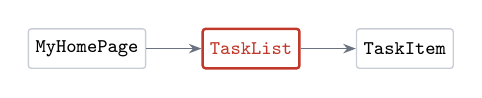
\begin{tikzpicture}[node distance=7mm]
        \node[o] (a) {MyHomePage};
        \node[o, nhanmanh, right=of a] (b) {TaskList};
        \node[o, right=of b] (c) {TaskItem};
        \draw[mt] (a) -- (b);
        \draw[mt] (b) -- (c);
      \end{tikzpicture}
    \end{column}
  \end{columns}
\end{frame}

\begin{frame}{3. Bảng so sánh}
  \small
  \renewcommand{\arraystretch}{1.45}
  \begin{tabular}{@{}>{\leavevmode\bfseries\color{chinh}}p{0.13\textwidth}@{\hspace{4mm}}P{0.38\textwidth}@{\hspace{5mm}}P{0.40\textwidth}@{}}
    \toprule
    Tiêu chí  & \textbf{Trạng thái cục bộ}\newline{\footnotesize\color{xam}Ephemeral state}
              & \textbf{Trạng thái cần chia sẻ}\newline{\footnotesize\color{xam}App state}\\
    \midrule
    Phạm vi   & Trong một widget đơn lẻ & Nhiều widget, nhiều màn hình\\
    Vòng đời  & Mất khi widget bị hủy (\ma{\footnotesize dispose})
              & Tồn tại suốt phiên sử dụng app\\
    Công cụ   & \ma{\footnotesize StatefulWidget} và \ma{\footnotesize setState}
              & \ma{\footnotesize InheritedWidget}, Provider, Riverpod, Bloc\\
    Ví dụ     & Con trỏ nhập văn bản, tab ảnh đang chọn
              & Giỏ hàng, tài khoản người dùng, theme\\
    Trong app & \ma{\footnotesize \_value} của \ma{\footnotesize TaskItem} ở Phần 2
              & \ma{\footnotesize \_tasks} ở \ma{\footnotesize MyHomePage}\\
    \bottomrule
  \end{tabular}
\end{frame}

% =====================================================================
\section{Kết luận}
% =====================================================================
\begin{frame}{Kết luận}
  \begin{enumerate}
    \setlength{\itemsep}{2.2mm}
    \item \textbf{State} là dữ liệu cần để dựng giao diện tại một thời điểm.
          Giao diện là kết quả của \ma{build} trên state.
    \item \textbf{Widget bất biến.} StatefulWidget tách thành hai class để dữ liệu
          thay đổi nằm trong object State sống lâu.
    \item \textbf{Vòng đời State} có ba giai đoạn: khởi tạo (\ma{initState} một lần),
          cập nhật (\ma{build} nhiều lần, sau mỗi \ma{setState}), giải phóng (\ma{dispose} một lần).
    \item \textbf{State cục bộ} để trong một widget, dùng \ma{setState}.
          \textbf{State cần chia sẻ} nếu chỉ dùng \ma{setState} sẽ gặp prop drilling,
          nên cần giải pháp quản lý tập trung.
  \end{enumerate}
\end{frame}

\begin{frame}{Tài liệu tham khảo}
  \small
  Kênh YouTube \textbf{Flutter} (Google):
  \vspace{2mm}
  \renewcommand{\arraystretch}{1.5}
  \begin{tabular}{@{}>{\color{chinh}\bfseries}l@{\hspace{4mm}}p{0.42\textwidth}@{\hspace{4mm}}>{\ttfamily\scriptsize\color{xam}}l@{}}
    Phần 1 & How do I make my first Flutter app & youtube.com/watch?v=xWV71C2kp38\\
    Phần 2 & What is State?                     & youtube.com/watch?v=QlwiL\_yLh6E\\
    Phần 3 & Stateful widgets in Flutter        & youtube.com/watch?v=Gzz8FwSlsUg\\
    Phần 4 & Managing State in Flutter          & youtube.com/watch?v=vU9xDLdEZtU\\
  \end{tabular}
  \vspace{3mm}

  Tài liệu Flutter:
  \begin{itemize}
    \item \emph{State class} (vòng đời State),
          {\ttfamily\scriptsize\color{xam}api.flutter.dev/flutter/widgets/State-class.html}
    \item \emph{Differentiate between ephemeral state and app state},
          {\ttfamily\scriptsize\color{xam}docs.flutter.dev/data-and-backend/state-mgmt/ephemeral-vs-app}
  \end{itemize}
  \vspace{2mm}

  Mã nguồn demo: thư mục \ma{chude10}, file \ma{lib/main.dart}.
\end{frame}

\end{document}
